\documentclass{article}
% packages
\usepackage[margin=1 in]{geometry}
\usepackage{indentfirst}
\usepackage{titlesec}
\usepackage{enumitem}

%math package
\usepackage{amsmath}
\usepackage{mathtools}

% Use Links
\usepackage{xcolor}
\usepackage[colorlinks=true ,citecolor=blue, urlcolor=blue,urlbordercolor={1 0 0}]{hyperref} 

\title{HUDM 5126 Linear Models and Regression Analysis Homework 1\footnote{This homework is written in \LaTeX.}}
\author{Yifei Dong}
\date{Sep 7 2020}

\begin{document}
\maketitle
\section{Grade Point Average}
\begin{enumerate}[label=(\alph*)]
\item Obtain the least squares estimates of $\beta_{0}$ and $\beta_{1}$, and state the estimated regression function.

$\beta_{0}=2.11405$, $\beta_{1}=0.03883$, $\overline{Y}=2.11405+0.03883*X$

\item Plot the estimated regression function and the data. Does the estimated regression function appear to fit the data well?

You can see the plot in Figure~\ref{fig:plot1}. The estimated regression function does not appear to fit the data very well since the R-squared was very low, which is 0.07262.

\begin{figure}[htbp]
\begin{center}
\caption{This is a scatter plot with the regression line.}
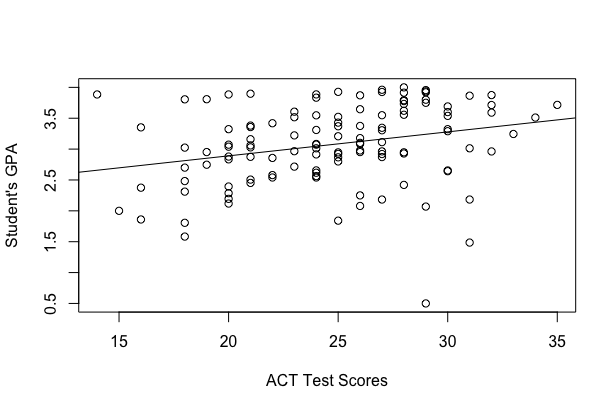
\includegraphics[width=100mm]{scatterplot.png}
\label{fig:plot1}
\end{center}
\end{figure}

\item Obtain a point estimate of the mean freshman GPA for students with ACT test score X=30.

$\overline{Y_{h}}=2.11405+0.03883*30=3.27895$

\item What is the point estimate of the change in the mean response when the entrance test score increases by one point?

For every one point increase in the entrance test scores, the grade point average (GPA) increases by 0.03883, which is $\beta_{1}$.

\end{enumerate}

\section{Least Squares Estimators}
\begin{equation} \tag{1.9a}
\sum Y_{i}=nb_{0}+b_{1}\sum X_{i}
\label{eq:1.9a}
\end{equation}

\begin{equation} \tag{1.9b}
\sum X_{i}Y_{i}=b_{0}\sum X_{i}+b_{1}\sum X_{i}^{2}
\label{eq:1.9b}
\end{equation}

\begin{equation} \tag{1.10a}
b_{1}=\frac{\sum (X_{i}-\overline{X})(Y_{i}-\overline{Y})}{\sum (X_{i}-\overline{X})^{2}}
\label{eq:1.10a}
\end{equation}

\begin{equation} \tag{1.10b}
b_{0}=\frac{1}{n}(\sum Y_{i}-b_{1} \sum X_{i})=\overline{Y}-b_{1}\overline{X}
\label{eq:1.10b}
\end{equation}
\begin{enumerate}[label=(\alph*)]
\item Derive the expression for $b_{1}$ in (\ref{eq:1.10a}) from the normal equation in (1.9).

First, solving \ref{eq:1.9a} for $b_{0}$, then
\begin{equation} \tag{1.32.1}
b_{0}=\frac{\sum Y_{i}-b_{1}\sum X_{i}}{n}
\label{eq:1.32.1}
\end{equation}

Similarly, solving \ref{eq:1.9b} for $b_{0}$, then
\begin{equation} \tag{1.32.2}
b_{0}=\frac{\sum X_{i}Y_{i}-b_{1}\sum X_{i}^{2}}{\sum X_{i}}
\label{eq:1.32.2}
\end{equation}

equating the results from \ref{eq:1.32.1} and \ref{eq:1.32.2}:
\begin{equation} \tag{1.32.3}
\frac{\sum Y_{i}-b_{1}\sum X_{i}}{n}=\frac{\sum X_{i}Y_{i}-b_{1}\sum X_{i}^{2}}{\sum X_{i}}
\label{eq:1.32.3}
\end{equation}

and then solving for $b_{1}$ yields:

\begin{equation} \tag{1.32.4}
b_{1}=\frac{n\sum X_{i}Y_{i}-\sum X_{i} \sum Y_{i}}{n\sum X_{i}^{2}-(\sum X_{i})^{2}}=\frac{\sum X_{i} Y_{i}-\frac{\sum X_{i} \sum Y_{i}}{n}}{\sum X_{i}^{2}-\frac{(\sum X_{i})^{2}}{n}}
\label{eq:1.32.4}
\end{equation}
\end{enumerate}

\end{document}



